\documentclass[bachelor, och, coursework]{shiza}
% параметр - тип обучения - одно из значений:
%    spec     - специальность
%    bachelor - бакалавриат (по умолчанию)
%    master   - магистратура
% параметр - форма обучения - одно из значений:
%    och   - очное (по умолчанию)
%    zaoch - заочное
% параметр - тип работы - одно из значений:
%    referat    - реферат
%    coursework - курсовая работа (по умолчанию)
%    diploma    - дипломная работа
%    pract      - отчет по практике
% параметр - включение шрифта
%    times    - включение шрифта Times New Roman (если установлен)
%               по умолчанию выключен
\usepackage{subfigure}
\usepackage{tikz,pgfplots}
\pgfplotsset{compat=1.5}
\usepackage{float}

%\usepackage{titlesec}
\setcounter{secnumdepth}{4}
%\titleformat{\paragraph}
%{\normalfont\normalsize}{\theparagraph}{1em}{}
%\titlespacing*{\paragraph}
%{35.5pt}{3.25ex plus 1ex minus .2ex}{1.5ex plus .2ex}

\titleformat{\paragraph}[block]
{\hspace{1.25cm}\normalfont}
{\theparagraph}{1ex}{}
\titlespacing{\paragraph}
{0cm}{2ex plus 1ex minus .2ex}{.4ex plus.2ex}

% --------------------------------------------------------------------------%


\usepackage[T2A]{fontenc}
\usepackage[utf8]{inputenc}
\usepackage{graphicx}
\graphicspath{ {./images/} }
\usepackage{tempora}

\usepackage[sort,compress]{cite}
\usepackage{amsmath}
\usepackage{amssymb}
\usepackage{amsthm}
\usepackage{fancyvrb}
\usepackage{listings}
\usepackage{listingsutf8}
\usepackage{longtable}
\usepackage{array}
\usepackage[english,russian]{babel}

%\usepackage[colorlinks=true]{hyperref}
\usepackage{url}

\usepackage{underscore}
\usepackage{setspace}
\usepackage{indentfirst} 
\usepackage{mathtools}
\usepackage{amsfonts}
\usepackage{enumitem}
\usepackage{tikz}

\newcommand{\eqdef}{\stackrel {\rm def}{=}}
\newcommand{\specialcell}[2][c]{%
\begin{tabular}[#1]{@{}c@{}}#2\end{tabular}}

\renewcommand\theFancyVerbLine{\small\arabic{FancyVerbLine}}

\newtheorem{lem}{Лемма}

\begin{document}

% Кафедра (в родительном падеже)
\chair{теоритических основ компьютерной безопасности и криптографии}

% Тема работы
\title{Сегментация изображений нейронными сетями}

% Курс
\course{2}

% Группа
\group{231}

% Факультет (в родительном падеже) (по умолчанию "факультета КНиИТ")
\department{факультета КНиИТ}

% Специальность/направление код - наименование
%\napravlenie{09.03.04 "--- Программная инженерия}
%\napravlenie{010500 "--- Математическое обеспечение и администрирование информационных систем}
%\napravlenie{230100 "--- Информатика и вычислительная техника}
%\napravlenie{231000 "--- Программная инженерия}
\napravlenie{100501 "--- Компьютерная безопасность}

% Для студентки. Для работы студента следующая команда не нужна.
% \studenttitle{Студентки}

% Фамилия, имя, отчество в родительном падеже
\author{Окунькова Сергея Викторовича}

% Заведующий кафедрой
\chtitle{доцент, к.ф.-м.н.} % степень, звание
\chname{М.~Б.~Абросимов}

%Научный руководитель (для реферата преподаватель проверяющий работу)
\satitle{Доцент} %должность, степень, звание
\saname{И. И. Слеповичев}

% Руководитель практики от организации (только для практики,
% для остальных типов работ не используется)
%\patitle{к.ф.-м.н.}
%\paname{М.~Б.~Абросимов}

% Семестр (только для практики, для остальных
% типов работ не используется)
%\term{8}

% Наименование практики (только для практики, для остальных
% типов работ не используется)
%\practtype{преддипломная}

% Продолжительность практики (количество недель) (только для практики,
% для остальных типов работ не используется)
%\duration{4}

% Даты начала и окончания практики (только для практики, для остальных
% типов работ не используется)
%\practStart{30.04.2019}
%\practFinish{27.05.2019}

% Год выполнения отчета
\date{2021}

\maketitle

% Включение нумерации рисунков, формул и таблиц по разделам
% (по умолчанию - нумерация сквозная)
% (допускается оба вида нумерации)
% \secNumbering

%-------------------------------------------------------------------------------------------
\tableofcontents

\intro

В наше время компьютеры стали очень важной частью наше жизни. Существует огромный пласт задач, решение 
которых мы уже не представляем без его использование. Поэтому не удивительно, что с каждым годом все больше 
и больше набирают популярность такие сферы, как нейронные сети, машинное и глубокое обучение. Данные направления
не просто способны решать большинство важных задач, но и делать это эффективно с помощью обучаемых систем, а
не программируемых.

Поэтому в данный момент одним из главных направлений в развитии IT-технологий является тема искусственного
интелекта и внедрение его во все сферы человеческой жизни. В некоторых областях искусственный интелект уже
превосходит человеческие возможности, так, например, уже существуют модели искусственного интелекта, которые
способны переиграть даже самых умелых шахматистов.

Нейронные сети и машинное обучение уже давно используются для решения многих бытовых задач: распознование и классификация 
объектов на изображении, классификация текста, распознование речи, выдача рекомендаций, основанных на наших предпочтениях, 
перевод текста с картинки и многих других. Одной из таких задач, а именно задаче сегментации изображения и посвящена 
данная работа.

Сегментацией изображения называют выделение однородных по некоторому критерию областей на изображении.
Таким образом, главной задачей сегментации, можно назвать разбиение изображения по заданному критерию 
на множества областей, которые у наблюдателя будут ассоциироваться с объектами на нашем исходном изображении 
или их частями, в результате которого на выходе получаются карты областей (сегментов). Иначе говоря, 
результатом сегментации является отображения множества точек изображения в множество итогового числа
разбиений на изображении. 

На практике чаще всего сегментацию исользуют для анализа медицинских изображений, например, для обнаружения 
различных опухолей и составлений рекомендаций по их лечению, выделения объектов на спутниковых снимках, 
распознования лиц или отпечатков пальцев, распознования дорожных знаков, для распараллеливание информационных 
потоков при передаче изображений высокого разрешения, а так же в сфере машинного зрения.

Задача сегментации неновая для человечества, потому ее иследованию было посвящено огромное количество 
научных работ. Благодоря чему сегодня существует много способов ее решения. В данной работе будут рассмотрены 
некоторые методы и алгоритмы машинного обучения для решения данной задачи, а также будут подробно описаны
принципы построения и обучения искусственных нейронных сетей. 

\section{Основные понятия и определения}

\textbf{Искусственный интелект (ИИ, AI, Artificial intelligence)} - это наука, описывающая создание машины или программы,
способной имитировать человеческое поведение для выполнения определенной задачи и обучаться за счет полученной в результате
работы информации.

Другими словами ИИ можно описать, как технологию, которая способна мыслить как человек и выполнять функции человека с большей
точностью. На практике же достаточно сложно создать идеальную модель ИИ, способного грамотно выполнять заданные ей функции. 
Поэтому для решения большинства задач в этой сфере используют машинное обучение.

\textbf{Машинное обучение (Machine learning, ML)} - это метод анализа данных, который автоматизирует построение аналитической 
модели.[1] Данная область ИИ воплощает в себе идею того, что машина способна обрабатывать полученные данные, анализировать их 
и на основе анализа обучаться с минимальным вмешательством человека.

Однака данная область ИИ всеже требует помощи в самом процессе обучения со стороны человека, а именно загрузку корректных данных,
рассматривающих все возможные случаи, на которых машина будет обучаться. Иначе говоря, несмотря на то, что данная система обучения
машины позволяет решить огромное количество задач, она не способна сама генерировать эти задачи.

\textbf{Глубокое обучение (глубинное обучение, Deep learning, DL)} - это тип машинного обучения, который обучает компьютер выполнять 
задачи человека.[1]

Данная система обучения вместо того, чтобы ждать тесты от человека, для дальнейшей их обработки по формулам, заданным изначально,
сама устанавливает начальные параметры и учит машину обучаться самостоятельно.

Таким образом, если представить AI, ML и DL в виде трех множеств, то мы получим картину, изображенную на рисунке 1:

\begin{equation}
    DL \subset ML \subset AI. 
\end{equation}

\begin{figure}[H]
    \centering
    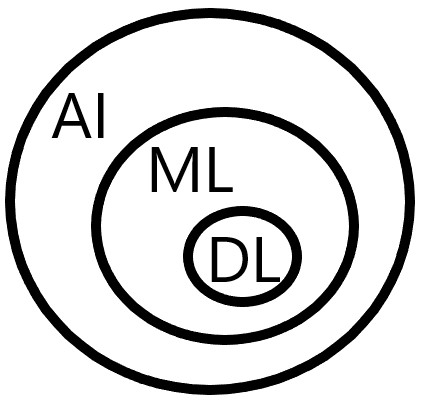
\includegraphics[width=0.35\textwidth]{2}
    \caption{Представление AI, ML и DL в виде множеств}
    \label{fig:img1}
\end{figure}

\textbf{Компьютерное зрение} - это одна из областей ИИ, которая отвечает за распознования компьютером визуального мира: фотографий и видео.
Оно подразумевает под собой методы, позволяющие обучить машину анализировать объекты и извлекать из этого какую-то информацию.

К задачам компьютерного зрения относятся:

\begin{enumerate}
    \item Классификация объектов на изображение.
    \item Сегментация изображения.
    \item Обнаружение объектов на изображение.
\end{enumerate}

Для решение задач в сфере машинного и глубокого обучения часто используют искусственные нейронные сети.

\textbf{Искусственные нейронные сети (ИНС, artificial neural networks, ANN)} - математическая модель и ее програмное воплощение, созданное
на основе модели биологических нейронных сетей (сетей нервных клеток организма).

ANN состоит из искусственных нейронов (ИН, artificial neuron, AN), являющихся програмной реализацией нейронов живых организмов и представляющих
из себя нелинейную функцию, называемую передаточной функцией, от массива входных данных ([$x_1, x_2, ..., x_n$]). Основная функция ИН - принятие 
входного сигнала с последующей его обработкой и передачей результата на другие нейроны.

Из всего выше описанного очевидно, что некоторые AN связаны между собой. Как и в биологии данную связь называют синоптической связью.

\textbf{Синапсом} в искусственных нейронных сетях называют связь между нейронами. По нему передаются выходные связи с одного нейрона на 
другой. У любого синапса имеется такой параметр, как весовой коэффициент $w_i$, который показывает текущее состояние нейрона, а более сложные 
синапсы также могут иметь память. Состояние нейрона в определенный момент времени вычисляется как взвешенная сумма его входов:

\begin{equation}
    s = \sum\limits_{i=1}^nx_iw_i,
\end{equation}
где n - число входов нейрона, $x_i$ - i-й входной сигнал, $w_i$ - вес i-го синапса.

В большинстве случаях связь между нейронами представляют в виде матрице W, которую соответственно называют матрицей веса.

Помимо синапсов важную роль в связи нейронов между собой играют аксоны. \textbf{Аксон} - это выходная связь нейрона, с помощью которой выходной 
сигнал нейрона поступает на синопсы других нейронов. Его значение будет равно:

\begin{equation}
    Y = f(s),
\end{equation}
где s - это состояние нейрона в данный момент, а f - это передаточная функция, в качестве которой чаще всего используются сигмоид, линейный порог,
гиперболический тангенс или жесткую пороговую функцию. Данная функция одинакова для нейронов одного слоя, но для нейронов разных слоев она могут
выбираться разные функции.

Проанализировав все выше описанное можно представить, как в общем выглядит нейрон:

\begin{figure}[H]
    \centering
    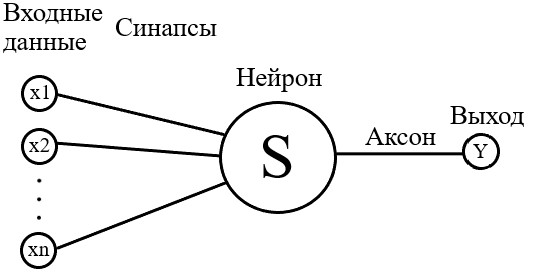
\includegraphics[width=0.5\textwidth]{3}
    \caption{Общий вид искусственного нейрона}
    \label{fig:img1}
\end{figure}

Уже на данном этапе достаточно информации, чтобы сделать вывод о том, как схематически можно изобразить искуственную нейронную сеть. Пример нейронной 
сети иозбражен на рисунке 3.

\begin{figure}[H]
    \centering
    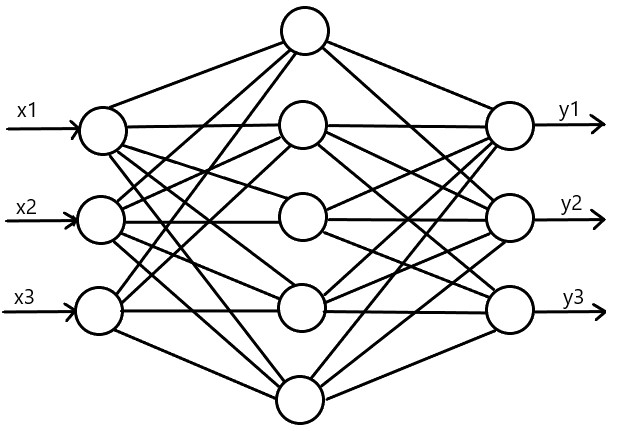
\includegraphics[width=0.55\textwidth]{4}
    \caption{Пример искусственной нейроннной сети}
    \label{fig:img1}
\end{figure}

\begin{center}
    \textbf{Обучение искусственной нейронной сети}
\end{center}

Как говорилось выше, для решения задачи не достаточно просто написать рабочую нейросеть, ее еще нужно и обучить. Под процессом обучения понимается выбор
таких параметров, при которых нейросеть решает поставленную задачу с большей эффективностью. Схема обучения изображена на рисунке 5. Математически его 
можно описать следующим образом. В процессе работа нейросеть, как было выясненно выше, формирует выходной сигнал Y = G(X), являющийся реализацией какой-то
функции. И пусть ответом на поставленную задачу будет функция Y = F(X), заданная с помощью параметра входных-выходных данных так, что

\begin{equation}
    Y^k = F(X^k),
\end{equation}
где k = 1, ..., N.

Обучением же будет состоять из генерации функции G(X), близкой к F(X). Оно будет состоять из множества итераций, на каждой из которых функция G(X) будет
все ближе и ближе к функции F(X), а для определения степени их близости друг к другу используют некоторую функцию $D_F(G)$, которую называют функцией ошибок или
целевой функцией. Таким образом обучение ИНС будет проходить до того момента, пока функция $D_F(G)$ не примет минимальное свое значение.

\begin{figure}[H]
    \centering
    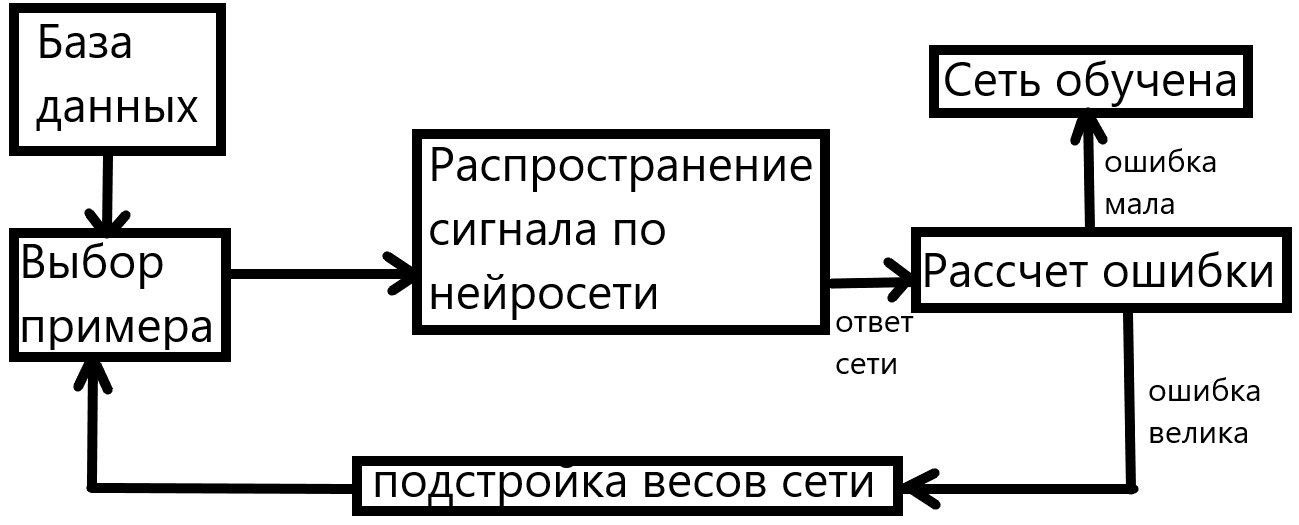
\includegraphics[width=0.85\textwidth]{5}
    \caption{Процесс обучения нейроннной сети}
    \label{fig:img1}
\end{figure}

Существует две главные стратегии обучения:

- с учитетелм или по другому контролируемое обучение (Supervised Learning)- нейросети на вход подаются данные и она обучается путем обработки этих данных;

- неконтролируемое обучение (Unsupervised Learning) - нейросеть обучается в соответствии с некоторым правилом, при этом данные для обучения не требуются;

Для обучения нейронной сети используют следующие типы алгоритмов:

\begin{enumerate}
    \item алгоритмы локальной оптимизации с вычислением частных производных первого порядка,
    \item алгоритмы локальной оптимизации с вычислением частных производных первого и второго порядка,
    \item стохастические алгоритмы оптимизации,
    \item алгоритмы глобальной оптимизации (задачи глобальной оптимизации решаются с помощью перебора значений переменных, от которых зависит целевая функция).
\end{enumerate}

\begin{center}
    \textbf{Сверточная нейронная сеть}
\end{center}

Наилучшие результаты в задачах распознования объектов на изображениях показала \textbf{сверточная нейронная сеть (Convolutional Neural Network, CNN, СНС)}, 
которую называют логическим продолжением идей когнитрона и некогнитрона. Главной причиной успеха данной архитектуры является учет двумерной тополгии изображения.
СНН работает по принципу маштабирования (свертки) изображения.

\textbf{Свертка} - это операция над матрицами A и B, размерностью  ($n_x * n_y$) и ($m_x * m_y$) соответственно, результатом которой является матрица C = A * B,
размер которой ($n_x - m_x + 1 * n_y - m_y + 1$), а элементы расчитываются по формуле:
\begin{equation}
    C_{i,j} = \sum\limits_{u=0}^{m_x-1}\sum\limits_{v=0}^{m_y-1}A_{i+u,j+v}B_{u,v}.
\end{equation}

\begin{figure}[H]
    \centering
    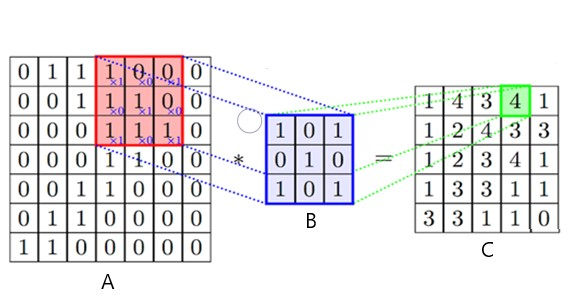
\includegraphics[width=0.85\textwidth]{6}
    \caption{Свертка}
    \label{fig:img1}
\end{figure}

Архитектура данного типа ИНС строится на чередовании слоев свертки и подвыборки, которые состоят из карт признаков. Они в свою очередь отвечают за поиск определенных
признаков. К примеру одна карта ищет предметы красного цвета, вторая - синего.

\section{Подходы к задаче сегментации изображения}

В данный момент выделяют два основных альтернативных друг другу подхода, которые используют алгоритмы сегменации изображений:

\begin{enumerate}
    \item Выделения границ областей;
    \item Наращивания точек области.
\end{enumerate}

Первый подход основан на том, что переход от одного объекта к другому на изображении происходит не плавно. Иначе
говоря, данный подход представляет из себя определение пикселей, которые находятся на границе двух областей 
изображения с дальнейшим выделением контуров(точек, между которыми происходит изменение яркости). Его очевидным 
плюсом является то, что помимо самих границ областей он позволяет идентифицировать и сами области. Ниже приведен
пример сегментации с помощью данного подхода.

\begin{figure}[H]
    \centering
    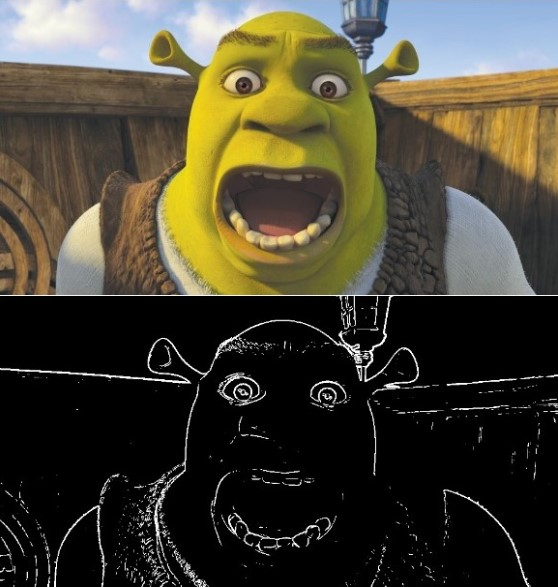
\includegraphics[width=0.5\textwidth]{1}
    \caption{Сегментация изображения с помощью выделения границ областей}
    \label{fig:img1}
\end{figure}

Второй подход наиболее распространенный и представляет из себя выделение точек на изображение, которые обладают 
одинаковыми свойствами, а после объединение их в область, которой присваивается смысловая метка. Именно данный
подход приимущественно используется в алгоритмах найросетей для решения задачи сегментации.

\begin{figure}[H]
    \centering
    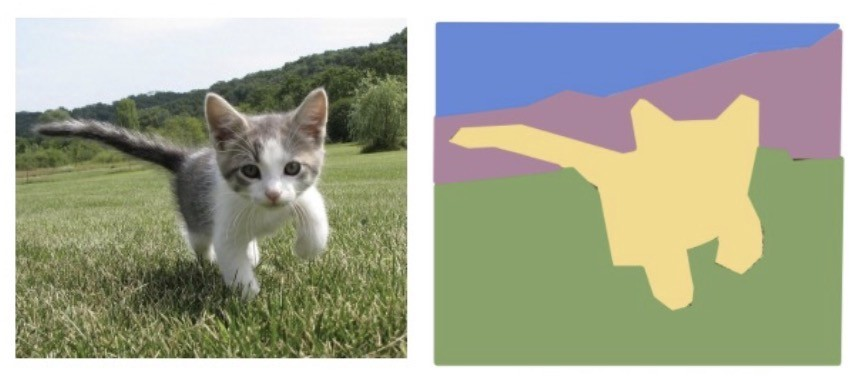
\includegraphics[width=0.7\textwidth]{7}
    \caption{Сегментация изображения с помощью наращивания точек области}
    \label{fig:img1}
\end{figure}

\section{Алгоритмы машинного обучения для решения задачи сегментациии изображения}

Для решение задачи сегментации изображения в основном выделяют следующие виды алгоритмов: 

\begin{enumerate}
    \item Пороговые алгоритмы; 
    \item Алгоритм наращивания областей; 
    \item Граничные алгоритмы;
    \item Алгоритмы сегментации на основе кластеризации.
\end{enumerate}

\subsection{FCN (fully convolutional network)}

Один из самых простых и наиболее распространенных алгоритмов искусственных нейронных сетей для сегментации изображения, который позволяет
работать с изображениями любого размера.

FCN представляет из себя полносверточную НС, которая за некоторое количество шагов выдает карту классов изображения. При этом на каждом шаге 
происходит свертка или транспонированная свертка изображения. На вход такая НС получает само изображение размерностью (W x H) и множество классов (C), к которым могут 
принадлежать пиксели с изображения. Первая часть слоев такой нейронной сети является реализацией уменьшения размерности (кодировки) с целью сбора контекстной
информации, а вторая часть - увеличения размерности (декодировки) с целью востановления пространственной информации, это связано с тем, что свертка матриц больших 
размерностей с большими количествами каналов является очень затратным процессом. В итоге размер изображения на входе равен размеру изображения на 
выходе. Конечная классификация выбирается поиском максимума по классам из многомерного массива, называемого тензором, который имеет размерность 
C x W x H. Для обучения такой ИНС используют функцию кросс-энтропии в качестве функции потерь для метода обратного распространения ошибок, имеющую вид:

\begin{equation}
    H(p, q) = -\sum\limits_{x}p(x)log(q(x)), 
\end{equation}
где p(x) - искомая вероятность, q(x) - действительная вероятность.

\begin{figure}[H]
    \centering
    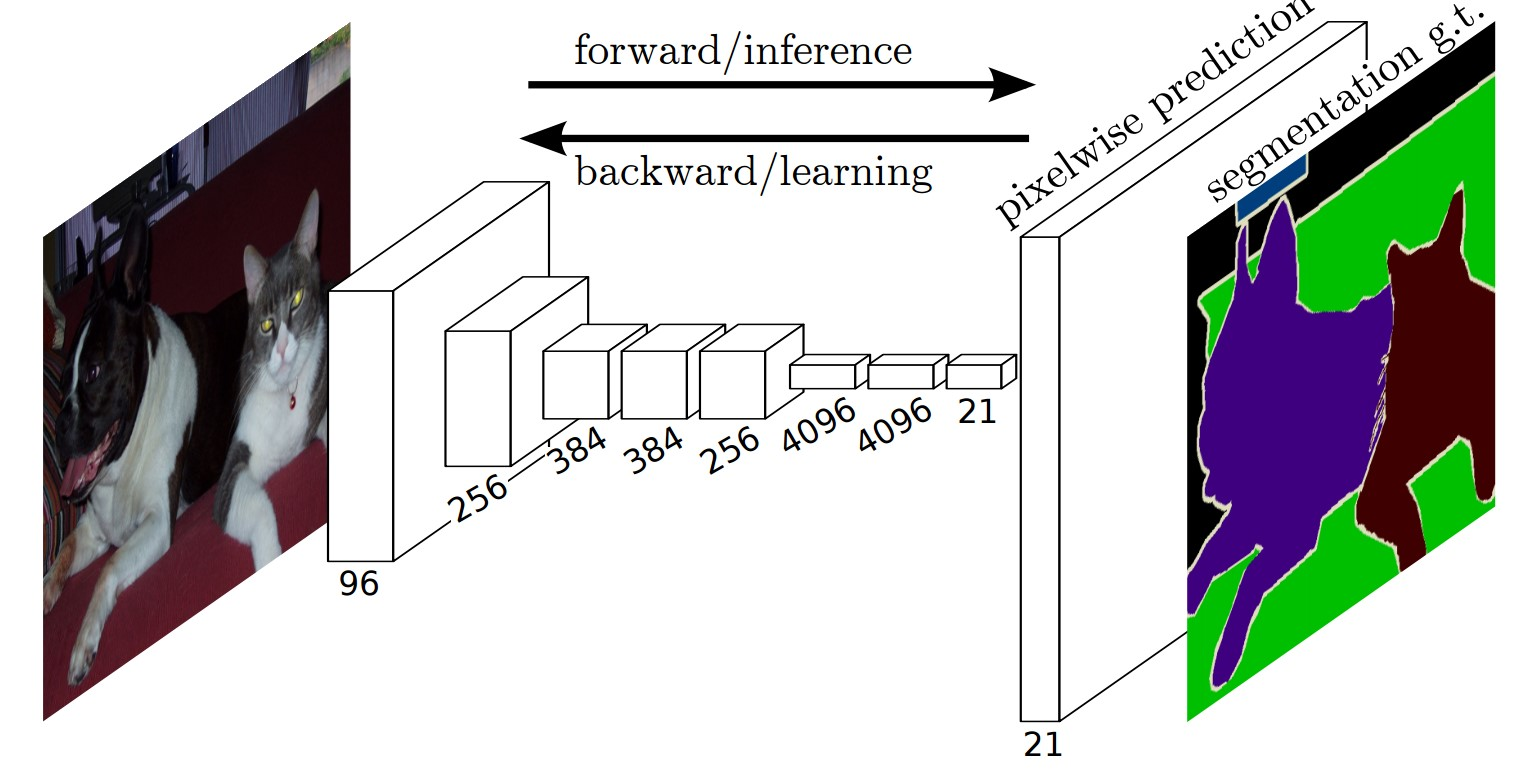
\includegraphics[width=0.6\textwidth]{9}
    \caption{Архитектура FCN[11]}
    \label{fig:img1}
\end{figure}

Не смотря на высокую эффективность имеет несколько болших не достатоков, главными из которых являются артефакты, расположенные в шахматном
порядке, появляющиеся всвязи с перекрытием выходов в операции транспонированной свертки, низкая разрешающая способность по краям, которая
обусловлена потерей информации во время кодирования, и отсутствие полностью связных слоев.

\subsection{U-Net}

На сегодняшний день U-Net считается одним из стандартов искусственных нейронных сетей для выполнения задачи сегментации изображения. ИНС типа 
U-Net представляют из себя улучшение архитектуры FCN. Свое название данная нейросеть получила за счет своей симетричной формы, отличающейся от 
других модификаций нейросети FCN. Главным различием между FCN и U-Net является наличие skip связей между выходами блоков уменьшения размерности 
и входами блоков увеличения размерности, находящихся на одном уровне, у последней, при этом очевидно, что за счет симетричной архитектуры количество 
блоков данных типов одинаково, что позволяет более точно передать информацию о свойствах каждого пикселя. Для обучения данной ИНС используется таже 
функция потерь, что и для обучения ИНС FCN.

Архитектуру U-Net можно разделить на 3 части:

\begin{enumerate}
    \item Путь кодировки,
    \item Узкое место, 
    \item Путь декодировки.
\end{enumerate}

\begin{figure}[H]
    \centering
    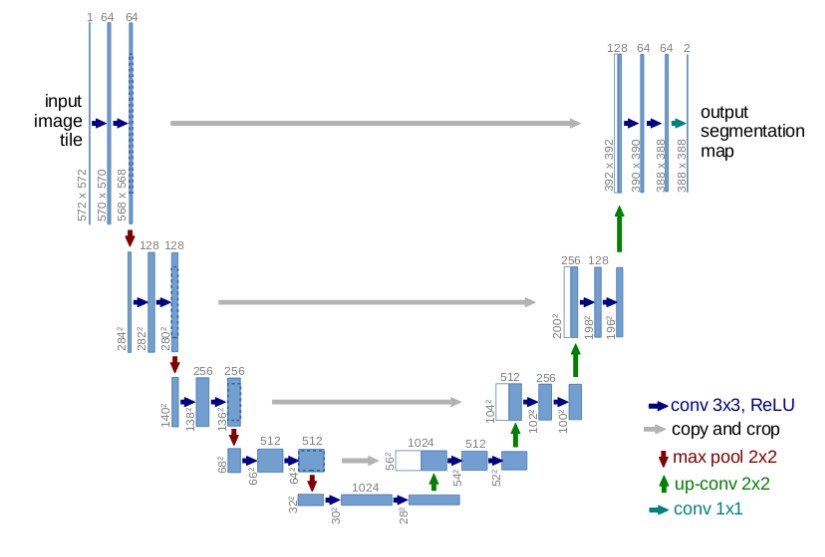
\includegraphics[width=0.7\textwidth]{8}
    \caption{Архитектура U-Net[9]}
    \label{fig:img1}
\end{figure}

Основное приимущество алгоритма U-Net является скорость по сравнению с другими алгоритмами сегментации изображения.

\subsection{Mask RCNN}

Данный алгоритм совмещает в себе два алгоритма: выше описанный FCN и Faster R-CNN, являющийся улучшением алгоритма Fast R-CNN, который в свою очередь 
является улучшением обычного R-CNN. 

\begin{figure}[H]
    \centering
    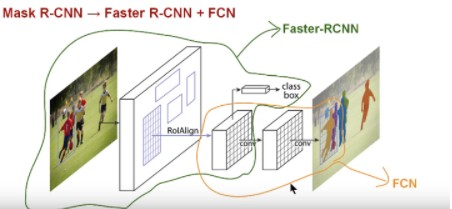
\includegraphics[width=0.85\textwidth]{10}
    \caption{Архитектура Mask RCNN[11]}
    \label{fig:img1}
\end{figure}

В основе Mask R-CNN лежит следующая архитектура:

\begin{enumerate}
    \item Изображение, поданное на вход нейроной сети, обрабатывается первым слоем. По итогу такой обработки получается карта признаков.
    \item Полученная карта передается следующему слою, на котором скользящее окно проходит по ней. По итоге данного шага выносится решение о наличии
    объекта в регионах.
    \item Результат предыдущего этапа передается на вход алгорима FCN, для определения более точного расположения объектаа на изображении.
\end{enumerate}

Функция потерь для данного алгоритма - это сумма потерь полученый во время процесса классификации, создании ограниченной области вокруг объекта и создании самой маски. Т.е. :

\begin{equation}
    L = L_{cls} + L_{box} + L_{mask}, где
\end{equation}
\begin{equation}
    L_{mask} = \frac{1}{m^2}\sum\limits_{1 \leq i, j \leq m}y_{ij}log(y_{ij}^k) + (1 - y_{ij})log(1 - y_{ij}^k),
\end{equation}
где k основной класс истинности.

Главным плюсом данного алгоритма является высокая точность вкупе с простым обучением и возможностью дообучить ИНС, но при этом сам процесс обучения
является весьма долгим.

\subsection{FRRN}

FRRN (Остаточные сети с полным разрешением ) - алгоритм многомерной двух поточной обработки, один из этих потоков называют остаточным, а другой - поток 
объединения. Первый из них отвечает за обработку карт объектов вполное разрешение, а второй сокращает их. Другими словами поток объединения работает с 
семантической информацией высокого уровня, а поток - с информацией пикселей низкого уровня.

При обучении данной ИНС, после каждого максимального пула, выполняется совместная обработка карт характеристик из каждого потока с целью объединения их информации.

Главный минус такого алгоритма является его затратность: обработка высокого разрешения требует значительное количество вычислительных ресурсов.

\begin{figure}[H]
    \centering
    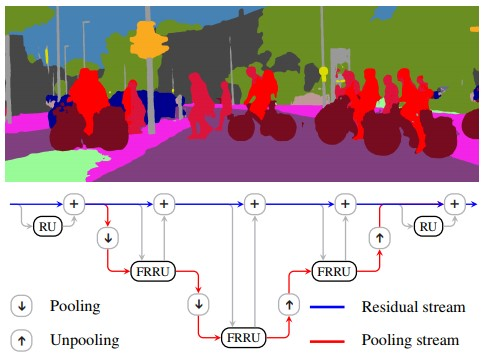
\includegraphics[width=0.45\textwidth]{11}
    \caption{Архитектура FRRN[12]}
    \label{fig:img1}
\end{figure}

\subsection{PSPNet}

Рассмотренный выше алгоритм FRRN является отличным примером маштабной обработки, имеющим свои плюсы и минусы. Алгоритм PSPNet в свое время предложил хороший 
способ обойти большинство главных минусов FRRN, который заключается в нескольких масштабах объединения. 

\begin{figure}[H]
    \centering
    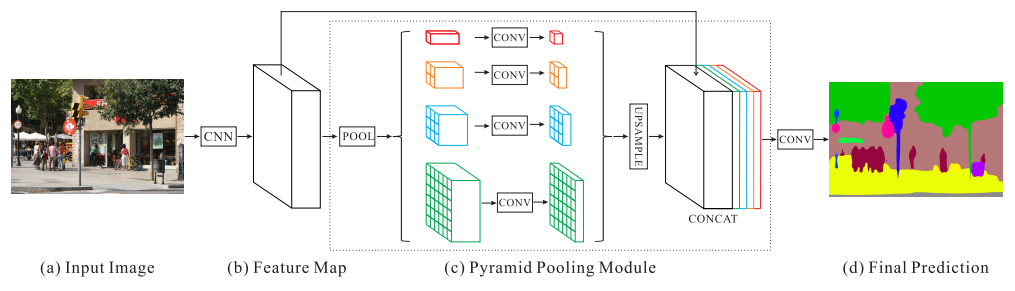
\includegraphics[width=1\textwidth]{12}
    \caption{Архитектура PSPNet[12]}
    \label{fig:img1}
\end{figure}

Реализация данного алгоритма как обычно начинается со стандартного извлечения признаков, а для дальнейшей обработки использует функции третьей понижающей 
дискретизации. Для получения многомасштабной информации алгоритм применяет четыре различные операции максимального пула к четырем различный размерам изображения, 
полученным на разных шагах, при этом не обрабатывая сами изображения, а после делает легкую свертку карты признаков каждого из них , объединяя их после и получая 
по итогу единую карту признаков, которую в свою очередь масштабируют до нужного размера с помощью билинейной интерполяции. Все это позволяет избежать реализации 
множества сверток, что решает проблему со временем выполнения данного алгоритма и затратностью.

\subsection{RefineNet}

Еще одним улучшением алгоритма FRRN можно назвать алгоритм RefineNet. Он так же работает с несколькими картами признаков объектов разномасштабных вариаций изображения, 
но делает это по принципу снизу вверх. Его главным плюсом является то, что он обрабатывает данные карты как по отдельности не зависимо друг от друга, так и вместе, благодаря
чему нужно обрабатывать и комбинировать вариации с низкими и высокими разрешениями.

\begin{figure}[H]
    \centering
    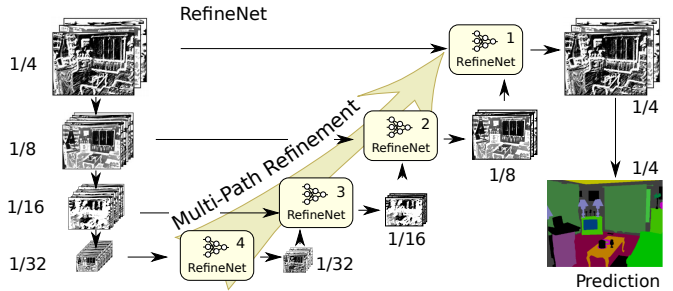
\includegraphics[width=0.8\textwidth]{13}
    \caption{Архитектура RefineNet[12]}
    \label{fig:img1}
\end{figure}

\subsection{GCN}

В нескольких предыдущих алгоритмах был рассмотрен такой процесс, как многомасштабная обработка. Однако в вышеописанных алгоритмах он выполнялся отдельно, а
результаты работы алгоритма впоследствии объединялись. Данный алгоритм решает этот вопрос, позволяя получить многомасштабную инффрмацию за один раз. Это
достигается за счет использование в данном алгоритме больших одномерных ядер вместо квадратных. Их главными плюсами являеся возможность эффективного масштабирования
и возможность обработки более одной шкалы за раз.

В остальном GCN работает по тому же принципу, что и другие алгоритмы его типа, но из-за эффективности одномерной свертки ему не нужно впоследствии масштабировать
обработанные разномасштабные вариации изображения, а достаточно просто выполнить обработку полноразмерного изображения. Это позволяет учитывать постоянное уточнение
сигментации по мере увеличения масштаба, а не сужение, которое может возникать в результате масштабирования.
\begin{figure}[H]
    \centering
    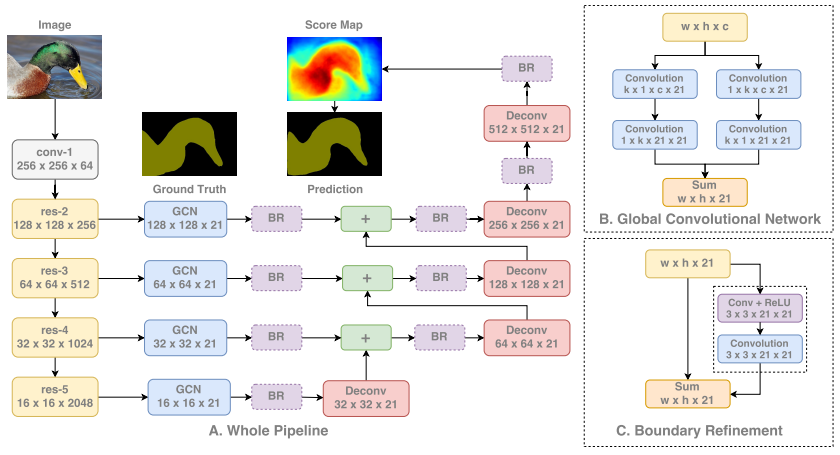
\includegraphics[width=1\textwidth]{14}
    \caption{Архитектура GCN[12]}
    \label{fig:img1}
\end{figure}


\newpage
\conclusion %заключение

В данной работе были рассмотрены следующие темы:

\begin{enumerate}
    \item Основная теоритическая информация о задачах искусственного интелекта, машинного и глубкого обучения, компьютерного зрения.
    \item Основы функционирования нейронных сетей и их обучения.
    \item Сверточные нейронные сети и процесс свертки.
    \item Краткая теории о задаче сегментации изображения и подходах ее решения.
    \item Алгоритмы ИНС для сегментации.
    \item Применение сегментации в жизни.
\end{enumerate}

В заключение данной работы нужно отметить, что сегментация изображения является очень важным средством для решения такого пласта задач, который связан с 
компьютерным зрением. Так как сегментация - это первый этап необходимый для анализа изображения. Поэтому с каждым годом появляется все больше и больше 
новых более оптимальных алгоритмов сегментации изображения. Подтверждение чего можно было увидеть в данной работе.

\begin{thebibliography}{3}
    \bibitem{1}
    Пять технологий искусственного интелекта, о которых вам нужно знать [Электронный ресурс] – URL: https://www.sas.com/ru_ru/insights/articles/analytics/five-ai-technologies.html (дата обращения 27.04.2021) - Загл. с экрана. Яз. рус.
    \bibitem{2}
    Нейронные сети для начинающих. Часть 1 [Электронный ресурс] – URL: https://habr.com/ru/post/312450/ (дата обращения 27.04.2021) - Загл. с экрана. Яз. рус.
    \bibitem{3}
    Нейронные сети — математический аппарат [Электронный ресурс] – URL: https://basegroup.ru/community/articles/math (дата обращения 27.04.2021) - Загл. с экрана. Яз. рус.
    \bibitem{4}
    Нейронные сети, или как обучить искусственный интеллект [Электронный ресурс] – URL: http://internetinside.ru/neyronnye-seti-ili-kak-obuchit-iskuss/ (дата обращения 28.04.2021) - Загл. с экрана. Яз. рус.
    \bibitem{5}
    Как работает нейронная сеть: алгоритмы, обучение, функции активации и потери [Электронный ресурс] – URL: https://neurohive.io/ru/osnovy-data-science/osnovy-nejronnyh-setej-algoritmy-obuchenie-funkcii-aktivacii-i-poteri/ (дата обращения 29.04.2021) - Загл. с экрана. Яз. рус.
    \bibitem{6}
    Сверточная нейронная сеть, часть 1: структура, топология, функции активации и обучающее множество [Электронный ресурс] – URL: https://habr.com/ru/post/348000/ (дата обращения 29.04.2021) - Загл. с экрана. Яз. рус.
    \bibitem{7}
    Сегментация изображения (Image segmentation) [Электронный ресурс] – URL: https://api-2d3d-cad.com/segment/ (дата обращения 29.04.2021) - Загл. с экрана. Яз. рус.
    \bibitem{8}
    Семантическая сегментация: краткое руководство [Электронный ресурс] – URL: https://neurohive.io/ru/osnovy-data-science/semantic-segmention/ (дата обращения 29.04.2021) - Загл. с экрана. Яз. рус.
    \bibitem{9}
    U-Net: нейросеть для сегментации изображений [Электронный ресурс] – URL: https://neurohive.io/ru/vidy-nejrosetej/u-net-image-segmentation/ (дата обращения 01.05.2021) - Загл. с экрана. Яз. рус.
    \bibitem{10}
    Семантическая сегментация - популярные архитектуры [Электронный ресурс] – URL: https://www.machinelearningmastery.ru/semantic-segmentation-popular-architectures-dff0a75f39d0/ (дата обращения 02.05.2021) - Загл. с экрана. Яз. рус.
    \bibitem{11}
    3 МЕТОДА ДЕТЕКТИРОВАНИЯ ОБЪЕКТОВ C DEEP LEARNING: R-CNN, FAST R-CNN И FASTER R-CNN [Электронный ресурс] – URL: https://python-school.ru/r-cnn-methods-for-object-detection/ (дата обращения 03.05.2021) - Загл. с экрана. Яз. рус.
    \bibitem{12}
    Семантическая сегментация с глубоким обучением [Электронный ресурс] – URL: https://www.machinelearningmastery.ru/semantic-segmentation-with-deep-learning-a-guide-and-code-e52fc8958823/ (дата обращения 02.05.2021) - Загл. с экрана. Яз. рус.
    
\end{thebibliography}

\end{document}